\documentclass[oneside,final]{report}

\usepackage{graphicx}
\usepackage[parfill]{parskip}

\graphicspath{{images/}}

\begin{document}
 

% ================ Front Matter ================
% Suppress page number for title page and letter of submittal
\pagestyle{empty}

% ==== Title Page
\begin{flushright}
 \begin{LARGE}
  \textbf{UNIVERSITY OF WATERLOO}
 \end{LARGE}

 \begin{large}
  Faculaty of Mechatronics Engineering\\[4cm]
 \end{large}

 \begin{LARGE}
  \textbf{
    Fourth Year Design Project \\[0.0cm]
    Final Design Report
  }
 \end{LARGE}

 \vfill

  Prepared By: \\[0.2cm]
  Iain Peet - 20252201\\
  Jordan Valentin - xxxxxxxx\\
  Rowan Head-Marsden - xxxxxxxx\\
  \today
\end{flushright}
\clearpage

% ==== Letter of Transmittal
\today \\[0.5cm]

Faculty of Mechatronics Engineering \\
University of Waterloo \\
Waterloo, Ontario \\

To Whom It May Concern:

Lorem ipsum dolor est... \\[0.5cm]

Sincerely, \\[1cm]

Iain Peet \hspace{4cm} Jordan Valentin \hspace{4cm} Rowan Head-Marsden
\clearpage

% Resume page numbering
\pagestyle{plain}
\setcounter{page}{1}
\pagenumbering{roman}

% ==== Table of Contents
\tableofcontents

% ==== List of Figures
\listoffigures
\addcontentsline{toc}{chapter}{List of Tables and Figures}

\chapter*{Executive Summary}
\addcontentsline{toc}{chapter}{Summary}

% ====================== Report Body =================================
\clearpage
\setcounter{page}{1}
\pagenumbering{arabic}
\pagestyle{headings}

\chapter{Introduction}

\section{Background}
Powered wheelchairs have obvious benefits for the mobility of the physically disabled.  As relatively heavy, powered vehicles, operation of these wheelchairs also carries obvious risk.  Thus, operators must be capable of safe operations.

Irene Ruel, a physiotherapist in the employ of the British Columbia Interior Health Authority, who has previously been responsible for powered wheelchair assessments in an extended care facilities, was consulted regarding this problem.  By her account, the risk that powered wheelchair operators will collide with other patients is a serious concern, which frequently results in the denial of requests for powered wheelchairs.

\section{Need Statement}
Access to powered wheelchairs may be restricted due to concerns about a patient's capability for safe operation.

\section{Objectives and Constraints}
The objectives of this design problem are as follows:

\begin{itemize}
 \item \emph{Improve safety}.  Safety is a significant concern for powered wheelchair operation.  Effective safety systems will be of great value to those with physical disabilities.
 \item \emph{Improve accessibility}.  For those who would be denied access to a powered wheelchair, a safety system which permits access will have significant quality-of-life benefits.
 \item \emph{Assist with difficult tasks}. Some tasks, such as precise positioning and movement in constrained spaces, are difficult even for unimpaired operators.   A system which can assist with such tasks would be helpful.
\end{itemize}

The constraints of the design are as follows:

\begin{itemize}
 \item \emph{Insensitive to operating environment}.  Realistic operating environments will be varied, and subject to change.  The usefulness of a safety system will be severely degraded if it depends on a specialized, controlled environment.
 \item \emph{Integrates with existing wheelchairs}.  Powered wheelchairs are expensive, and many are already in existence.  The potential reach of a new safety system will be severely restricted if it may not be integrated with pre-existing wheelchairs.
 \item \emph{Cost kept below \$500}.  The system will be paid for by end users, who will be sensitive to cost.  It will be difficult to market a system which is very expensive relative to the cost of a basic powered wheelchair.
\end{itemize}

\section{Criteria}
% TODO(rowan)

\section{Patents}
% TODO(jordan)


\chapter{Proposed Solution}

\section{Mechanical Designs}
% TODO(rowan)

\section{Mechanical Design Selection}
% TODO(rowan)

\section{Sensor Selection}
% TODO(rowan)

\section{Sensor Configuration}
% TODO(iain)

\section{Sensor Configuration Selection}
%TODO(iain)


\chapter{Detailed Design}

\section{Summary}
%TODO(?)

\section{Mechanical Design}
%TODO(rowan)

\section{Systems Integration}
%TODO(iain/jordan)

\section{Software Design}
%TODO(iain/jordan)

\chapter{Schedule and Budget}
%TODO(rowan)

\section{Schedule}
\begin{figure}[htb]
 \centering
 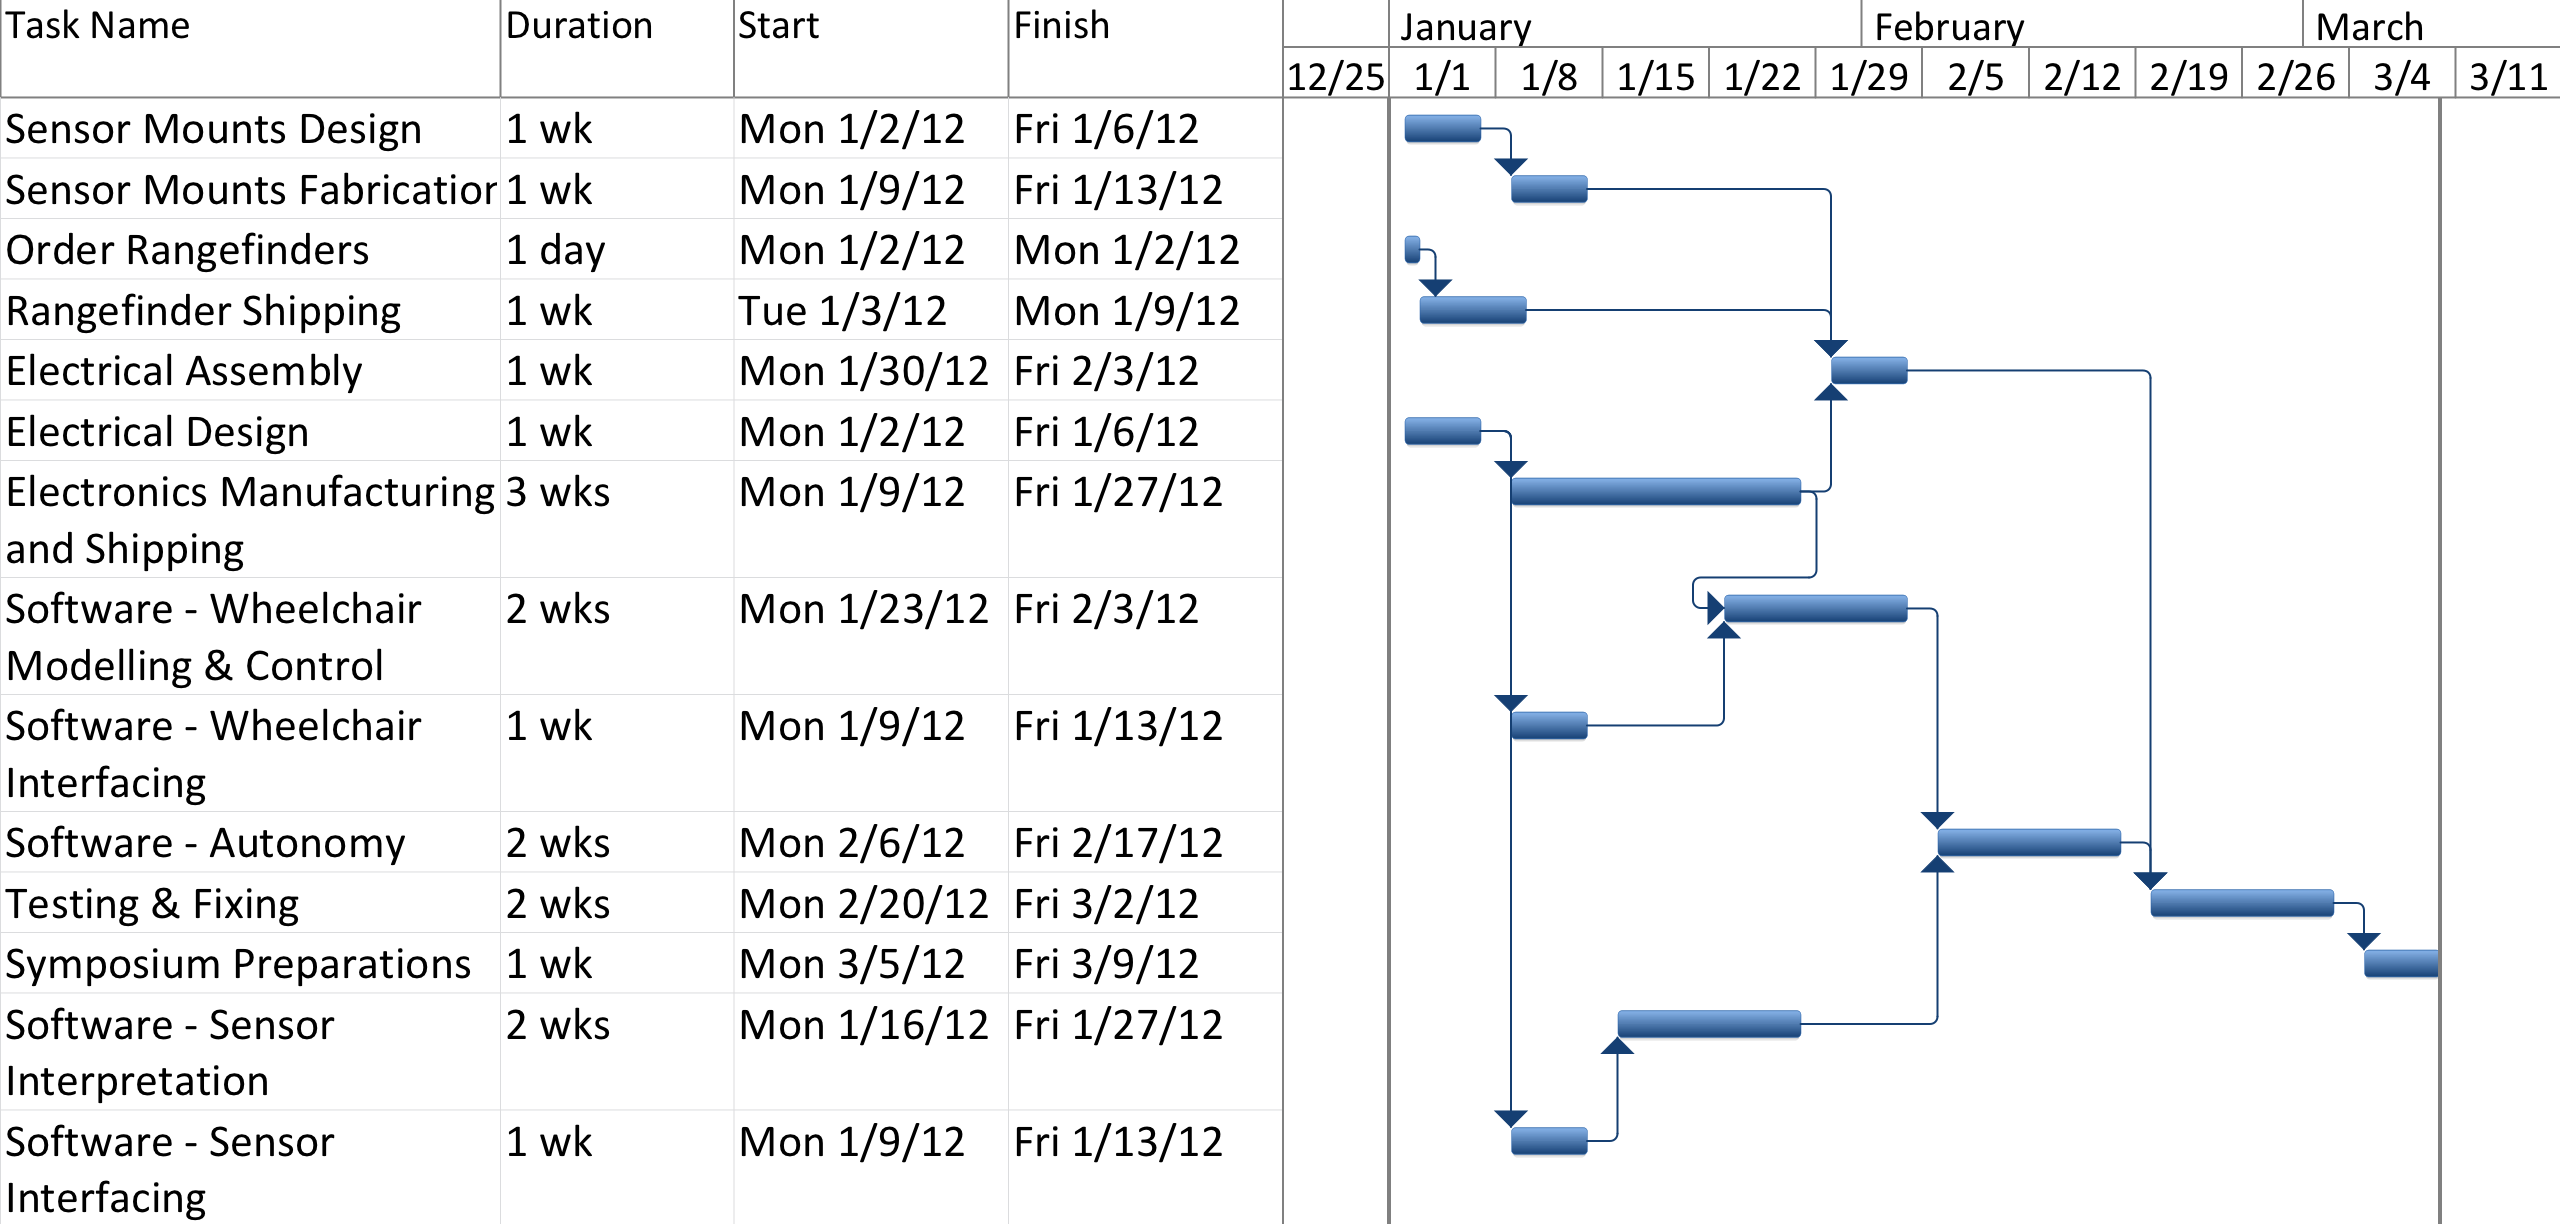
\includegraphics[scale=0.6]{gantt.png}
 \caption{Production schedule for the prototype}
 \label{schedule}
\end{figure}

Figure \ref{schedule} shows the prototype production gantt chart.  It may be seen that the prototype is expected to be completed about a week before the March 19 symposium.  The timeline is dominated by electrical and software tasks; if possible, it would be especially advantageous to begin electrical design work early.

\section{Bill of Materials}
\begin{table}[t]
\centering
\begin{tabular}{|l|c|c|c|}
\hline
Part & Count & Cost (CAD) & Total (CAD) \\
\hline
Xbox Kinect & 1 & 150 & 150 \\
\hline
Xbox Kinect Mount & 1& 15 & 15 \\
Sonar Sensor & 4 & 30 & 120 \\
\hline
Sheet Metal & 1 & 12 & 12 \\
\hline
Spacers & 8 & 0.25 & 2 \\
\hline
PCB \& Components & 1 & 150 & 150 \\
\hline
Basic Netbook & 1 & 250 & 350 \\
\hline
\hline
Total&&&789\\
\hline
\end{tabular}
\caption{Bill of Materials}
\label{tab:BOM}
\end{table}


\chapter{Conclusions and Recommendations}
%TODO(?)

\chapter*{Appendix A}
\addcontentsline{toc}{chapter}{Appendix A - Patents}
%TODO(jordan)

\begin{thebibliography}{9}
 \addcontentsline{toc}{chapter}{Bibliography}

 % NB: cite these with \cite{item}

 \bibitem{lv-ez4}
   \emph{LV-EZ4 Datasheet}, MaxBotix Inc, 2011
\bibitem{kinect_accuary}
L. Yiping. “openni\_kinect/kinect\_accuracy” Internet: http://www.ros.org/wiki/openni\_kinect/kinect\_accuracy, Jun. 27, 2011.
\bibitem{kinect_power }
	M. Wise. “Adding a Kinect to an iRobot Create.” Internet: http://www.ros.org/wiki/kinect/Tutorials/Adding\%20a\%20Kinect\%20to\%20an\%20iRobot\%20Create, May 2, 2011.
\bibitem{patent:power_wheelchair}
	G. Griggs, T. Dutta, G. Fernie. “Powered Wheelchair.” U.S. Patent 2010/0082182A1, Apr. 1, 2010.
\bibitem{patent:wheelchair_method}
	T. Smithers, U. Urriticoechea, U. Campos. “Wheelchair and Method for Correcting the Guidance of a Wheelchair.” U.S. Paten 2011/0130940A1, Jun. 2, 2011.
\bibitem{patent:computer_controlled}
	L. Fehr, S. Skaar, G. Del Castillo. “Computer Controlled Power Wheelchair Navigation System.” U.S. Paten 2008/7383107B2, Jun. 3, 2008.
\bibitem{MSP430_USB}
	A. Dannenberg. (2006, October). MSP430 Connectivity Using TUSB3410. Available: http://www.ti.com/lit/an/slaa276a/slaa276a.pdf
\end{thebibliography}


\end{document}